\documentclass[a4paper]{jsarticle}
\usepackage{amsmath,amsfonts}
\usepackage{bm}
\usepackage{siunitx}
\usepackage[dvipdfmx]{graphicx}
\usepackage[dvipdfmx]{color}
\usepackage{listings}
\usepackage{ascmac,url}

\newcommand{\var}[1]{\texttt{#1}}

\begin{document}
\begin{titlepage}
\begin{center}
\vspace*{150truept}
{\huge アセンブリ言語 期末課題 レポート}\par
\vspace{50truept}
{\large 講義名:アセンブリ言語}\par
\vspace{5truept}
{\large 学籍番号:23B30032}\par
\vspace{5truept}
{\large 氏名:飯田悠太}\par
\vspace{5truept}
{\large 作成日:\today}
\end{center}
\end{titlepage}
本レポートは,アセンブリ言語の期末課題であるcalc0からcalc3までの4つのバージョンの電卓コンパイラそれぞれについて,実装方法とその工夫,考察について述べるものである。
\section{calc0}
この章ではcalc0の実装,つまり課題であるcalc1からcalc3までのアセンブリを出力するベースとなるCのコードについて述べる。
\subsection{全体の実装}
入力された式については\var{p}というポインタ型の変数に格納し,これを先頭から1文字ずつ\var{while}で読んでいくことにより,電卓の入力を1文字ずつ読んでいくということを再現した。

入力された要素については,数字,演算子,メモリキー,符号反転キーの4つに分類して処理することにした。また,演算結果を処理するための変数として,現在入力されている数値を管理する変数\var{num}と,演算子を管理する変数\var{lastOp},現在までの計算結果を管理する変数\var{acc},メモリ機能の値を管理する変数\var{mem},符号反転キーが入力された回数を管理する変数\var{countS}を用意した。

以下,入力要素の種類ごとの処理について述べる。
\subsubsection{数値の管理}
数値については,数字が入力されるたびに既存の\var{num}を10倍し,それに現在見ている数字\var{*p}から'0'を引いたものを加えることで,数値を管理することにした。これは,10進数の数値の表現方法をそのまま利用したものであり,簡単に理解することができる。文字型から数値への変換には,数字に連続されたコードが与えられるというASCIIコードの性質を利用している。

\subsubsection{演算子の管理}
もし現在見ている文字が演算子(\var{+}, \var{-}, \var{*}, \var{/}, \var{=})である場合,まず見ている文字の次の文字が演算子でなくなるまでポインタを進める。これは,電卓で言うところの「最後に入力された記号キー」を拾ってきて,それ以外の演算子の入力は無視する,という動作を実現するためである。

演算子の入力が確定した時点で,今入力された演算子ではなく,元々持っていた演算子で計算を行う。これは,演算を行うためには,演算子の前までの計算値と演算子の直後にくる数値の2つが必要であるが,演算子を見た時点では演算子直後の数値が確定していないので,代わりに前回の演算子の前までの計算値と前回の演算子,そして前回の演算子直後の数値を用いて計算する必要があるからである。それゆえ,\var{lastOp}の初期値は\var{+}としておく必要がある。なぜならば,式中で初めて演算子を見た時に行うべき計算は\var{acc}に\var{num}を代入するという操作であり,その操作は\var{acc}の初期値0に\var{num}を加えるという操作と等価であるからである。

また,符号の反転については,\var{num}の符号について,\var{countS}が偶数の時には符号を反転し,奇数の時には反転しないようにすることで,符号反転キーが押された回数に応じて符号を反転することができる。

計算を終えた後,現在見ている演算子を\var{lastOp}に代入し,\var{num},\var{countS}を0にリセットする。これにより,次の数値の入力に備えることができる。

\subsubsection{メモリ機能の管理}
メモリ管理機能について,まず,\var{C}が入力された場合は\var{mem}に\var{acc}の値を代入し,\var{R}が入力された場合は,\var{acc}に\var{mem}の値を代入するようにしている。これらは非常にシンプルである。

次に,\var{P},つまりメモリ加算キーが入力された場合について考える。この場合,まず\var{P}が入力される前までの演算結果を用意する必要があるので,\var{P}が入力された時点での\var{acc}, \var{num}, \var{lastOp}, \var{countS}の値に基づいて演算を行う。そしてその値を\var{mem}に加算する。これにより,メモリ加算キーが入力された時点までの計算結果をメモリに保存することができる。すると,\var{mem}以外の各種変数が保持している値はもはや必要がなくなる(なぜならばメモリに保存されているから)ので,これらは全て初期値にリセットする。

\var{M},つまりメモリ減算キーが入力された場合の動作は,\var{mem}への加算が減算に変わるだけで,\var{P}の場合とほぼ同様の処理を行うことで実現できる。

\subsection{実装の工夫点}
この実装で工夫した点は\var{lastOp}の初期値を\var{+}にした上で,演算子を遅延処理するようにしたことである。これにより,最初の数値入力も含めて全て同一の方法で処理することができ,コードの可読性向上につながっている。

\section{calc1}
この章ではcalc1の実装について述べる。なお,実装のベースの考え方はcalc0と同様であるので,本章ではcalc0でのC言語ベースの実装をどのようにアセンブリに落とし込んだかについて述べる。

\subsection{変数の取り扱い}
まず,課題のレギュレーションの制約上,calc0ではC言語の変数として管理していた\var{num}, \var{acc}, \var{mem}, \var{countS}を,アセンブリで管理する必要がある。そこで,\var{acc}はレジスタ\var{eax}, \var{num}はレジスタ\var{ecx}で管理し,\var{mem}と\var{countS}はスタックで管理することにした。

このように設計した理由を述べる。そもそも,アセンブリコードを書き始めた時はこれら4つの変数は全てレジスタで管理していた。しかしながら,コードを書き進めるうちに,使用するアセンブリが混雑してきたり,誤ってcallee-saveなレジスタをスタックへの退避なしで使用してしますミスが発生してしまったりすることがあると気づいた。そこで,比べて使用頻度の少ない\var{mem}と\var{countS}をスタックで管理し,使用するタイミングでのみスタックから取り出して空いているレジスタに読み込んだり,直接アドレスを参照するようにした。また,\var{num}と\var{acc}に割り当てるレジスタの選定であるが,\var{acc}は最終的な式の計算結果が格納されることが期待されるため,関数の返り値の格納に使われる\var{eax}を使用することにした。\var{num}を格納するレジスタについては,caller-saveなレジスタのうち\var{eax}でないもの,という理由で\var{ecx}を選択した。

また,このコード上では変数に0を代入する操作を頻繁に行うが,多くの部分で単に\var{mov}命令で即値0を代入するのではなく,\var{xor}命令を用いて0クリアを行うようにした。これは,\var{mov}命令による即値代入よりも\var{xor}命令を用いた方が高速であるという知見を得たからである。また,そのような背景があるため0クリアには\var{xor}命令を用いることが一般的であるという言説を聞き,慣例に則った方がより読み手に理解されやすいだろうと思い\var{xor}を用いたという側面もある。これもコードの工夫と言えるだろう。

\subsection{数値の管理}
数値の取り扱いについては,calc0で説明した実装を単純にアセンブリに置き換えて行ったのみである。

\subsection{演算子の管理}
演算子の管理について,まず\var{lastOp}についてはレギュレーション上C言語での管理が認められていたので,calc0通りの実装のまま行った。

それ以降の処理について述べる。まず初めに符号反転キーの処理を行うことにした。符号反転キーが押された回数は常にスタックの上から2番目に置かれているので,これを空いている\var{rdx}レジスタに読み込む。その後\var{testb}命令を使うことにより,$\var{rdx} \&\& 1$の結果が0であるかどうか,つまり符号反転キーが押された回数が偶数か奇数かを判定するようにした。これにより,ゼロフラグがセットされている時,つまり符号反転キーが偶数回押されている時は数値の符号を反転させる\var{negl}命令をジャンプするようにした。以上のようにして,符号反転キーの処理を行った。

ここで,ジャンプ用のラベルとして1, というのを用いているが,これは数値ラベルである。これを用いた理由は,この命令は複数回出力されるため,グローバルラベルを用いるとラベル名の衝突によるエラーが発生してしまうからである。

また,その後の演算は\var{lastOp}に記録された演算子に対応するアセンブリ命令を用いるだけであるが,割り算の場合においては若干実装に工夫があるので,それについて述べる。
割り算のとき,負数の取り扱いのために符号拡張を行う必要がある。講義資料では\var{eax}レジスタの正負に合わせて\var{mov}命令により\var{edx}の上位ビットをセットする方法が紹介されていたが,今回は\var{cltd}命令を用いた。これにより,割り算の際に\var{eax}の符号に合わせて\var{mov}命令でセットする値を変更する,というコードを書かなくて良くなり,コードが簡潔になった。

\subsection{メモリ機能の管理}
メモリ機能の管理については,calc0で述べた実装をそのままアセンブリに置き換えたのみである。メモリの値についてはスタックの先頭に積むことにしたので,メモリの値を書き換える必要がある時は\var{rdx}レジスタに読み出して処理を行ったのち,スタックに積み直すようにした。

\subsection{その他の部分}
コードの終了部分では,計算結果を返すために,講義資料で示された例に従ってprintfを呼び出している。また,資料の例ではプログラムの終了のために\var{ret}命令を用いていたが,今回はexitを呼び出すことでプログラムを終了させるようにした。
コードの終了部分の工夫として,スタックに積んでいた\var{mem}と\var{countS}をポップするために,\var{pop}命令ではなく\var{add}命令を用いてスタックポインタを移動させるようにしたことが挙げられる。スタックポインタが指すアドレスをデータ2つ分スタックの下に移動することにより,\var{pop}命令を2回書かずともスタックの先頭2つのデータを削除することができる。

\section{calc2}
この章ではcalc2の実装について述べる。calc2ではcalc1での実装をベースに,オーバーフロー検知や0割り検知を行うようにした。本章では,calc1から変更された実装について述べる。

\subsection{オーバーフロー検知}
オーバーフローの検知は,演算子の処理部分で各演算子に対応する命令を実行した後と数値入力の処理のための命令を実行した後に\var{jo overflow}を使用することで行う。これにより,種々の計算によってオーバーフローフラグがセットされた時に,オーバーフロー時の対応を行うための処理ブロックにジャンプすることができる。

\var{overflow}ラベル以下での処理は以下の通りである。まず,\var{leaq}命令によりエラーメッセージ(今回は単にEのみ)をセットし,\var{call}命令でprintfを呼び出してエラーメッセージを表示する。その後,exitステータスとして1をセットした上で\var{call}命令でexitを呼び出してプログラムを終了させる。

\subsection{0割り検知}
0割りの検知は,\var{idiv}命令を実行する前に\var{cmpl \$0, \%ecx}と\var{je division\_by\_zero}を実行することで0割りの検知を行う。\var{cmpl}命令を実行することで,\var{ecx}がゼロであればゼロフラグがセットされるので,その次の\var{je}命令で条件分岐することができる。

division\_by\_zero以下の処理は,オーバーフロー検知時と同様である。

\section{calc3}
この章ではcalc3の実装について述べる。calc3では,calc1の実装をベースに\var{imull}命令と\var{idiv}命令を用いずに乗除を表すことを目指した。本章では,calc1から変更された実装について述べる。

\subsection{乗算の実装}
\var{imull}を用いない乗算について,正数同士の掛け算と符号の処理に分けて実装した。

まず,正数同士の掛け算の実装について説明する。この実装では,\var{ecx}に格納されている乗数と\var{eax}に格納されている被乗数を用いて,ビットシフトとキャリーフラグを用いることで乗算を実現している。少し込み入った手順であるため,以下に番号付き箇条書きで用いた命令とその意図について述べる。

\begin{enumerate}
    \item \var{rcrl \$1, \%ecx}: 乗数\var{ecx}を1ビット右回転させる。この操作により,乗数の最下位ビットがキャリーフラグ(CF)に移動する。これは,掛け算の筆算での,下一桁を取り出して,その掛け算を考えるという動作を実現するためである。
    \item \var{jnc 3f}: CFがクリアであれば,次の加算処理をスキップする。これは,乗数の最下位ビットが0の場合は被乗数に0を掛ける処理をすることになり,そのような処理は最終的な値に影響を与えないからである。
    \item \var{addl \%eax, \%edx}: CFがセットされている場合(乗数の最下位ビットが1の場合),結果を保持するレジスタ\var{edx}に被乗数\var{eax}を加算する。
    \item \var{shll \$1, \%eax}: 被乗数\var{eax}を1ビット左シフトする。これは,乗数の次の桁に対応するための処理である。2進数では,桁が1つ左にシフトすると値が2倍になるため,乗算における桁上がりを表現できる。筆算で言えば,桁ごとの掛け算の結果ごとに一つずつ位をずらして書くという操作に相当する。
    \item \var{testl \%ecx, \%ecx} and \var{jnz 2b}: 乗数\var{ecx}が0になるまで,ステップ1から4を繰り返す。\var{ecx}が0になるということは見るべき桁がなくなったこと,つまり乗数の全てのビットを処理したことを意味する。また,この命令によりCFはクリアされる。
\end{enumerate}


上記の動作について,図\ref{fig:mul_example}に示すような例($11 \times 5 = 55$)を用いて説明する。


\begin{figure}[h]
    \centering
    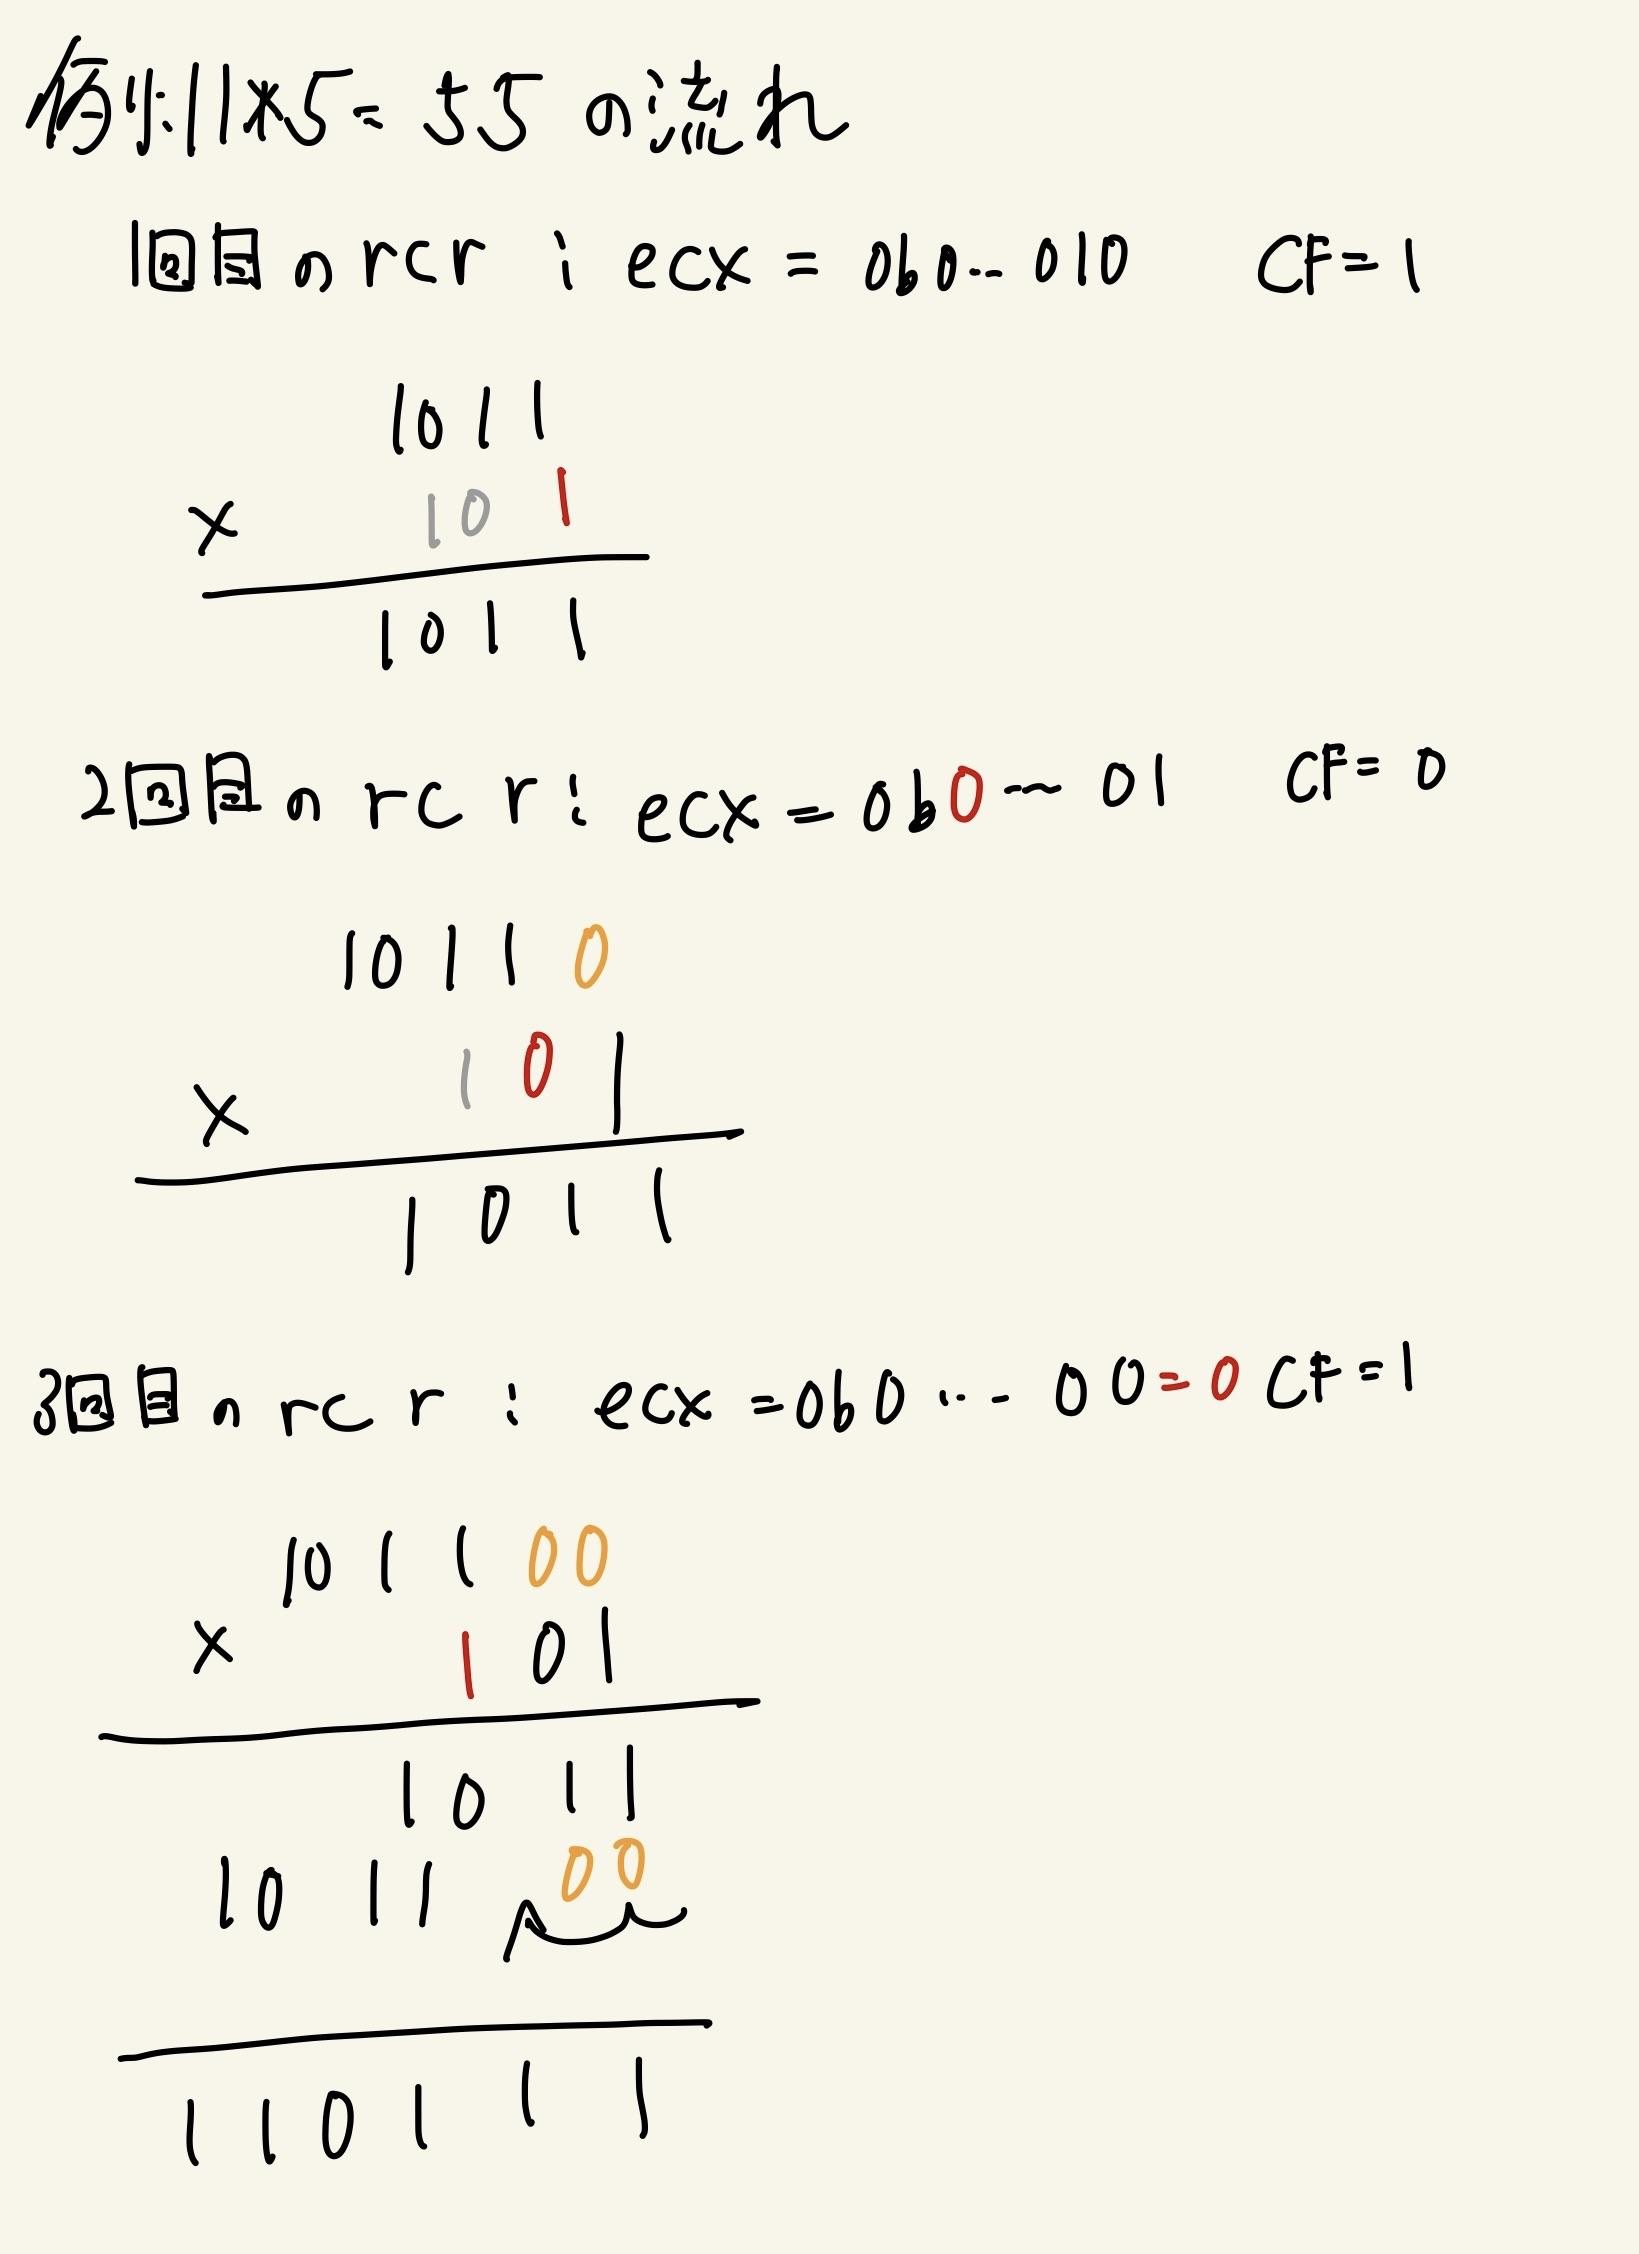
\includegraphics[width=8cm]{./img-mul.jpg}
    \caption{ビットシフトによる掛け算の動作例}
    \label{fig:mul_example}
\end{figure}


まず,1回目の\var{rcr}命令により,乗数の1桁目の数字がわかる。この場合,乗数の1桁目は1であるため,\var{addl}命令により被乗数を\var{edx}に加算する。また,それに続いて\var{shl}命令により被乗数を1ビット左シフトしておく。

2回目の\var{rcr}命令により,乗数の2桁目が0であるということがわかり,\var{addl}命令はスキップされる。また,2回目の\var{rc}命令の前に\var{test}命令を実行しているため,キャリーフラグがリセットされている故,\var{ecx}の最上位ビットは1ではなく0になっていることに注意する。その後,\var{shl}命令により被乗数を1ビット左シフトしておく。

3回目の\var{rcr}命令により,乗数の3桁目が1であるということがわかり,\var{addl}命令により被乗数を\var{edx}に加算する。ここで,これ以前に被乗数は2回左シフトされているが故に,足し込まれる値も最初と比べて2ビット分左にずれており,これが筆算の位取りを表していることがわかる。

今回は3回\var{rcr}命令を実行すると\var{ecx}が0になるので,ここで掛け算の作業は終了し,答えとして\texttt{110111\textsubscript{2}}$=55$が得られる。

続いて,符号処理の実装方法について考える。calc2までのように先んじて乗数の符号を変えてしまうと,2の補数表現を用いている間係でうまくいかないケースが出てきてしまうと考え,乗数と被乗数の符号をまとめて処理することにした。
具体的な実装としては,まず,\var{test}命令を用いることで,被乗数\var{eax}の符号をチェックする。もし被乗数が負の数であれば,\var{negl}命令を用いて被乗数を正の数に変換すした上で,countSをインクリメントする。そして乗算が終了したタイミングで,計算結果の正負をcountSに応じて調整する。こうすることで,被乗数の正負の情報をcountSに渡し,まとめて処理することができる。

以上のような\var{imull}を用いない乗算の実装のポイントは,乗数の最下位ビットを見るために\var{rcr}命令を用いたことである。これにより,例えばシフトしてから\var{and}命令を用いるなどの余分な動作をせず,短いコードで確実に乗算を行えるようになった。また,掛け算の筆算における,各桁ごとの掛け算の結果を1桁ずつずらして書いて最後に足しこむ,という動作を被乗数を左シフトすることにより実装したことは,かなり直感的で分かりやすい実装であると考えている。

また,被乗数と乗数の符号の情報をcountSにまとめ,最後に処理するという実装も,最も大変な掛け算の実装のロジックに複雑な場合分を入れなくて済むという点で優れている。

\subsection{除算の実装}

\var{idivl}を用いない除算について,乗算と同様に正数同士の割り算と符号の処理に分けて実装した。

まず,正数同士の割り算の実装について説明する。この実装では,\var{eax}に格納されている被除数,\var{ecx}に格納されている除数を用いて,ビットシフトと減算を用いることで除算を実現している。以下に番号付き箇条書きで用いた命令とその意図について述べる。

\begin{enumerate}
\item \var{xorl \%edi, \%edi}:部分剰余を格納するレジスタ\var{edi}を0クリアする。
\item \var{movl \%ecx, \%edx}:除数\var{ecx}の値を\var{edx}にコピーする。\var{ecx}はループカウンタとして使用するため,除数の値を保持するために\var{edx}を用いる。
\item \var{movl \$32, \%ecx}:ループカウンタ\var{ecx}に32を設定する。カウンタを32にするのは,除算を行うために1ビットずつ見ていく必要があるからであり,かつ今回は32ビット整数を扱うからである。
\item \var{xorl \%esi, \%esi}:商を格納するレジスタ\var{esi}を0クリアする。
\item \var{shll \$1, \%eax}:被除数\var{eax}を1ビット左シフトする。
\item \var{rcll \$1, \%edi}:\var{eax}の最上位ビットをキャリーフラグを介して\var{edi}に移動させる。これは,被除数のビットを1つずつ取り込んでいく処理であり,これは割り算の筆算で上の桁から一桁ずつずらして商が立つところを探す動作に相当する。
\item \var{shll \$1, \%esi}:商\var{esi}を1ビット左シフトする。これは,割り算の筆算で数字を立てる桁を一つずつ下にずらしていく動作に相当する。
\item \var{cmpl \%edx, \%edi}:\var{edi}と除数\var{edx}を比較する。
\item \var{jl 3f}:
\var{edi}が除数より小さい場合,次の減算処理をスキップする。
\item \var{addl \$1, \%esi}:\var{edi}が除数以上の場合,商\var{esi}に1を加算する。これは,割り算の筆算で数字を立てることに相当する。
\item \var{subl \%edx, \%edi}:\var{edi}から除数\var{edx}を減算する。
\item \var{decl \%ecx}:ループカウンタ\var{ecx}をデクリメントする。
\item \var{testl \%ecx, \%ecx} and \var{jnz 2b}:ループカウンタ\var{ecx}が0になるまで,ステップ5から12を繰り返す。また,この命令によりCFはクリアされる。
\end{enumerate}

\begin{figure}[h]
    \centering
    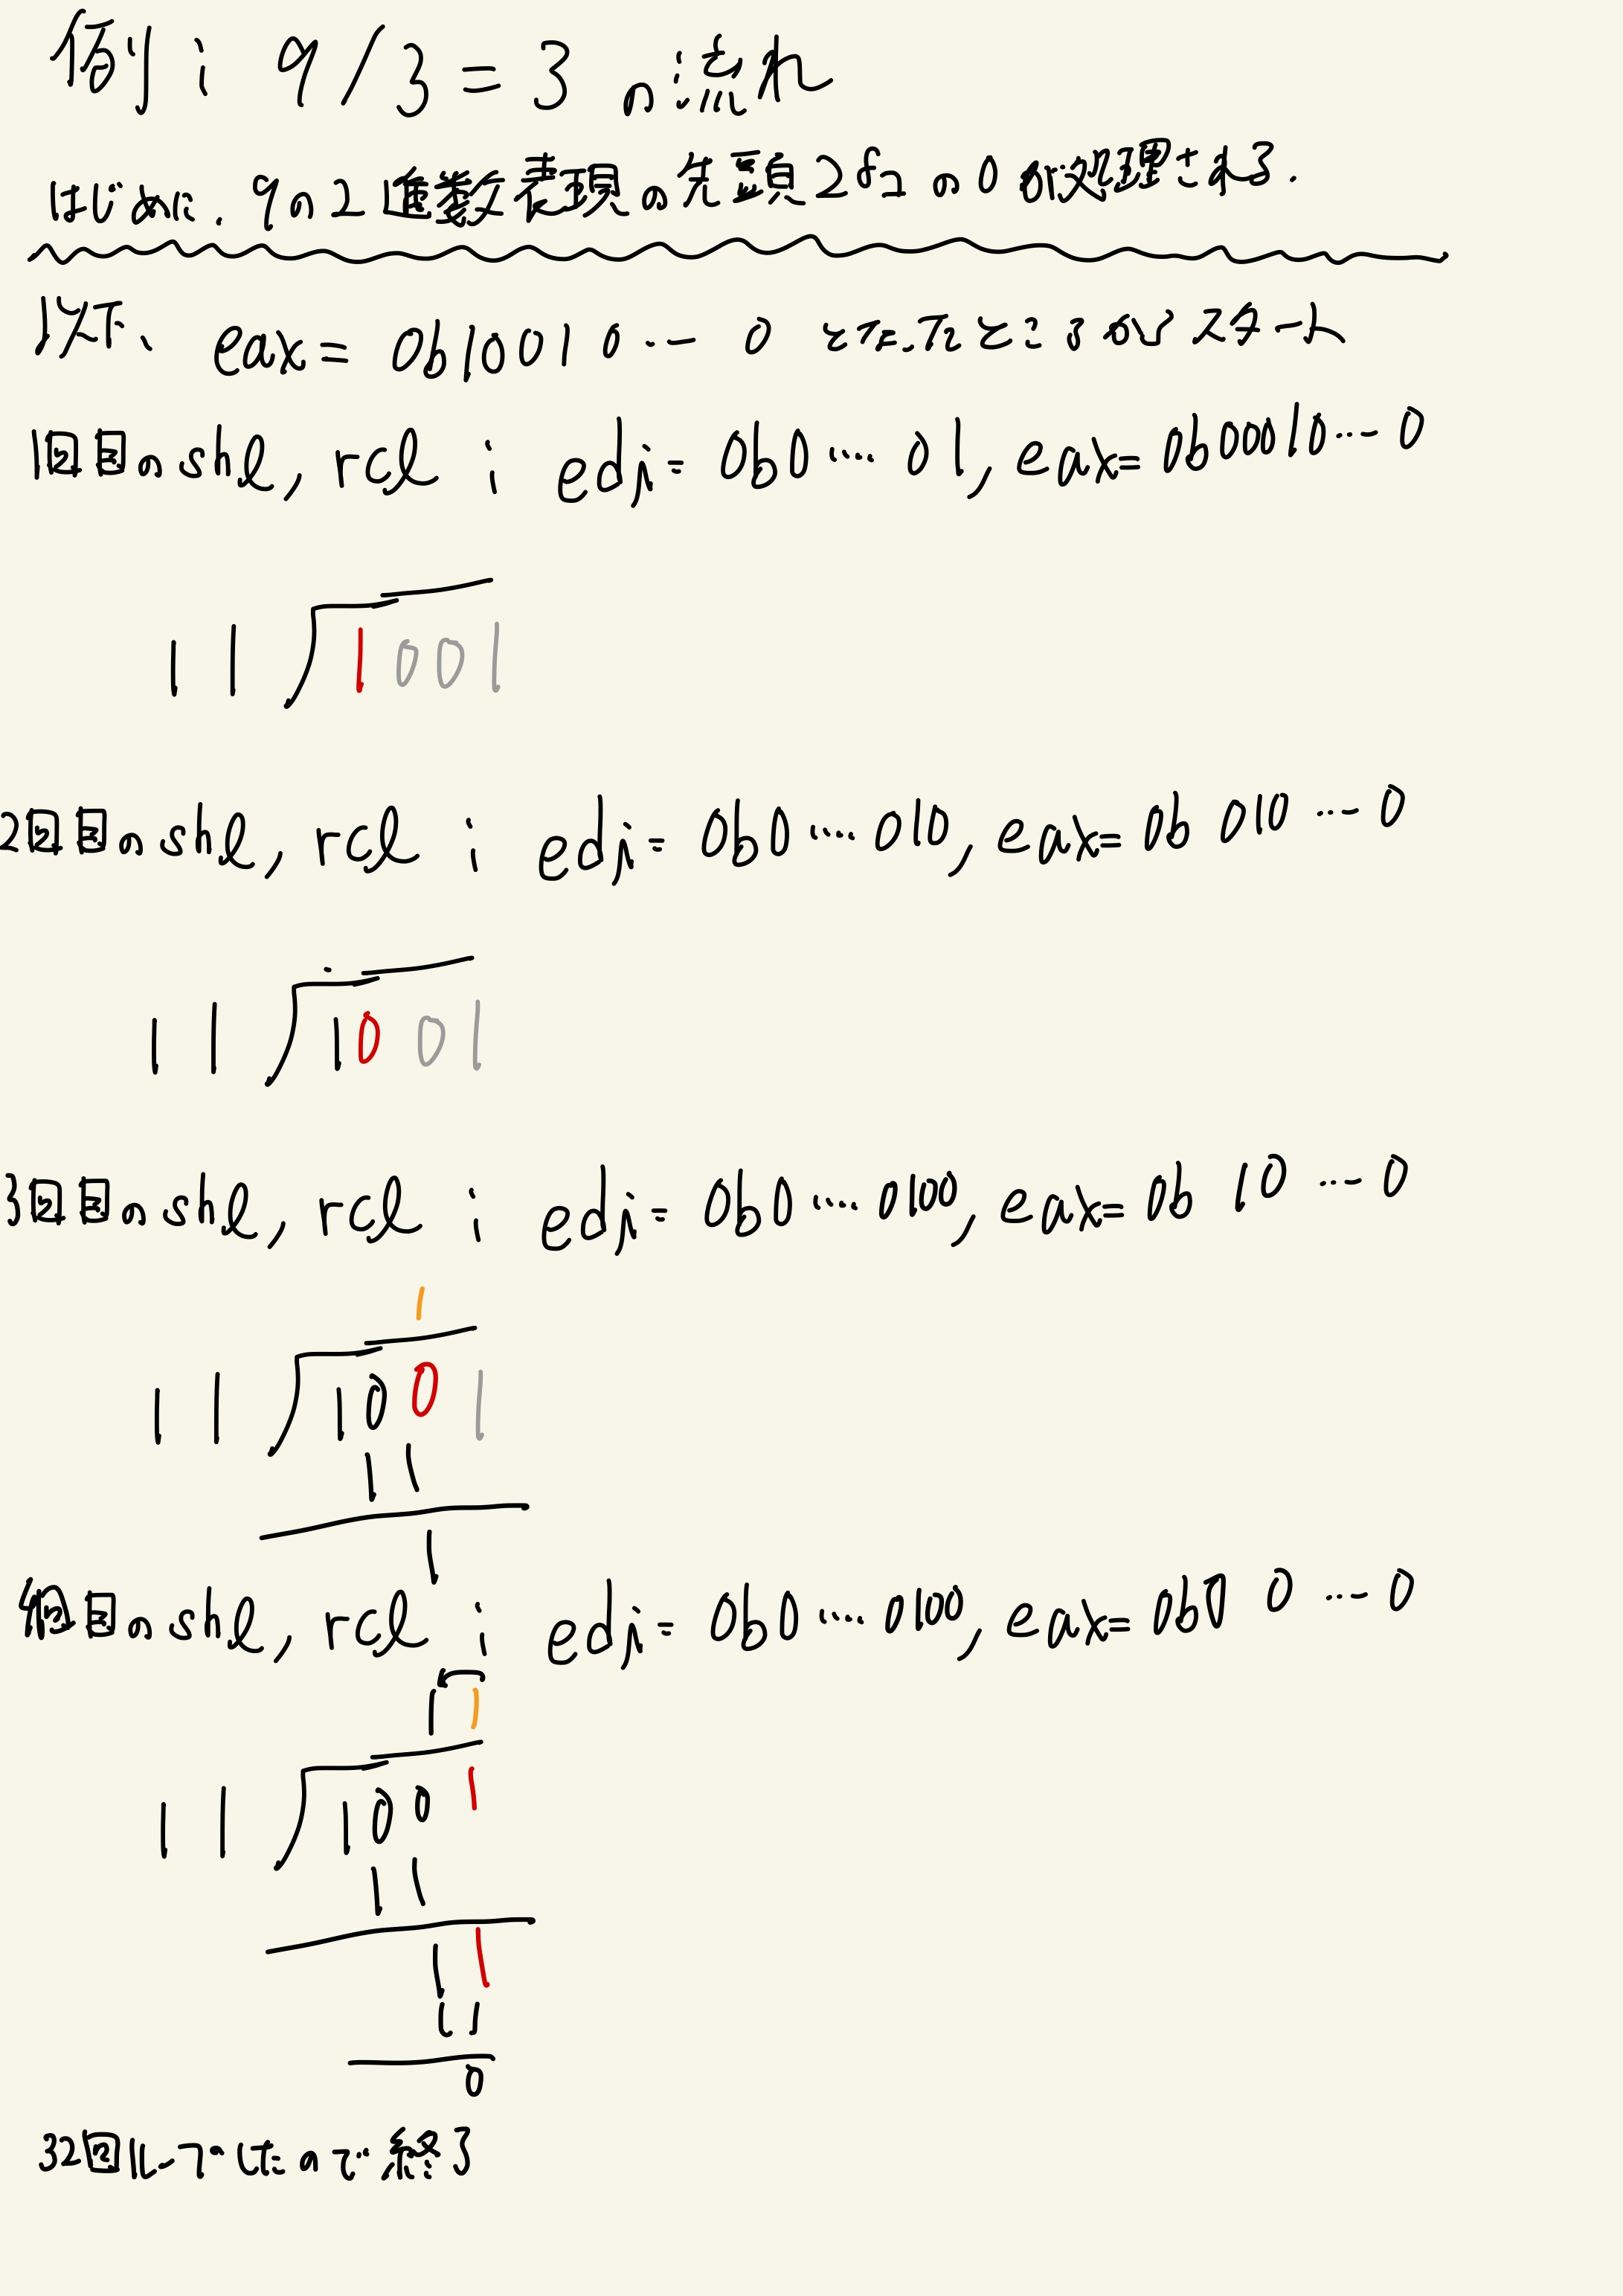
\includegraphics[width=10cm]{./img-div.jpg}
    \caption{ビットシフトによる割り算の動作例}
    \label{fig:div_example}
\end{figure}


上記の動作のうち,割り算のロジックに直接関連するステップ5以降について,図\ref{fig:div_example}に示すような例($9 / 3 = 3$)を用いて説明する。

ここで,$9 = 0\var{b}0\cdots01001$であり,9の二進数表記の先頭28個は0である。これは\var{shl}命令が28回実行されることにより,特に結果に影響を与えずスキップされる。なぜならば,先頭の0を取り出してそれを\var{edi}に移している間,\var{edi}の値は0で,常に除数よりも小さいためである。よって,以下の説明では28回ループを回した後から説明する。

まず,29回目の\var{shl}命令と\var{rcl}命令により,CFを通じて1が移動し,\var{edi}の値が1となる。この時,まだ除数の方が大きいため,減算処理はスキップされる。このような動作は,割り算の筆算を行う時に商に数字が立つかどうかを上から一桁ずつ見ていく動作に相当する。その後,\var{shl}命令が実行される。これは,そこまでに立てていた商を1つシフトすることで,位取りの動作を再現するためである。

次に,30回目の\var{shl}命令と\var{rcl}命令により,\var{edi}の値が2となる。この時,まだ除数の方が大きいため,減算処理はスキップされる。

次に,31回目の\var{shl}命令と\var{rcl}命令により,\var{edi}の値が4となる。この時,除数が\var{edi}以下になったので,商に1を立てるために\var{esi}に1を加算する。その後,\var{subl}命令により,\var{edi}から除数を減算する。これは,割り算の筆算において商に数字が立った時にそこまでの段階で見ている数から除数を引く動作に相当する。

最後に,32回目の\var{shl}命令と\var{rcl}命令により,\var{edi}の値が11となる。この時,除数が\var{edi}以下であるので,商に1を立てるために\var{esi}に1を加算する。その後,\var{subl}命令により,\var{edi}から除数を減算する。

これによりループが終了し,結局答えとして\texttt{11\textsubscript{2}}$=3$が得られる。


続いて,符号処理の実装方法について説明する。乗算の場合と同様に,被除数と除数の符号をまとめて処理するために,被除数の符号を\var{test}命令でチェックし,負の数であれば\var{negl}命令で正の数に変換し,countSをインクリメントする。そして除算が終了したタイミングで,計算結果の正負をcountSに応じて調整する。

以上のような\var{idiv}を用いない除算の実装のポイントは,乗算の場合と同様に,\var{rcl}命令によるシンプルな手法に被除数の値を見ることができる点である。また,これらの動作は割り算の筆算の手法を直感的に表現しており,理解しやすい実装であると考えている。

\section{より良いテストケースの提案}
この章では,私の実装に合わせてテストケースをどのように修正したかについて述べる。

まず,calc3で符号入れ替えの処理を加減算と乗除算で使い分けたため,


\section{全体の実装についての反省・考察}
この章では,私の実装を振り返り,その良し悪しや改善すべき点について考察する。

初めに,良かった点について述べる。まず,calc1からcalc3までそれぞれに課せられた課題を達成することができた(少なくとも配布+自分で設定したテストケースが全て通った)ことについては満足している。既知のバグなども存在していない。

また,calc3の乗算や除算の実装については,ローテート命令を適切に活用することにより,掛け算/割り算の筆算を直感的に実装できたことは比較的よい実装ができたと言えるだろう。

一方で,このコードには課題が多くある。第一に,レジスタとスタックの使い方に課題があるだろう。今回の私の実装では,累積値と途中に入力された数値はレジスタで管理しており,また演算子についてはC言語で管理していた。しかしながら,講義の資料で紹介された木構造による計算式の処理では入力された記号を木構造で管理し,数値をpushし,記号が来たらpopしてその記号に応じた計算をするというような実装をしていた。

私の実装は今回のようにコードが行う動作が限定的であれば問題ないが,より複雑な作業を行ったり複数の作業をする必要があったりする場合には,レジスタの数が不足してしまい,不足するたびにスタックに値を積む必要が生じ,スタック上の値の管理が煩雑になってしまうだろう。一方で講義で紹介された実装であれば,常に記号が来るたびに2つの数をpopして計算しその結果をpushするという処理を繰り返すだけでよいため,無駄なレジスタを使用することがなく,またスタックの管理も簡単になるであろうと考えられる。よって,授業で紹介された方法の方が,拡張性という点で私の実装よりも優れていると考えられる。

また,コードの実行速度についても疑問がある。例えばレポート中で,\var{xor}命令による0クリアは\var{mov}命令によるものよりも高速であると知られている,というように述べたが,これは実際に計測した結果ではなく,環境によって異なる可能性も十分に考えられる。よって,よりより設計をするためには計測が不可欠であると考えるが,私は本課題でそれを怠ってしまった。文献や口伝による情報を信じるばかりでなく,実際のユースケースにおける計測を行うことが重要であるのだから,それをするべきであった。

さらに,前に述べた内容と関連する部分もあるが,私のコードはまだC言語に依存している部分が多いと感じる。例えば式の入力や演算子の管理はC言語で行なったり,C言語で出力するアセンブリの条件分岐を行ったり,関数呼び出しを行ったりしている。これらの部分をアセンブリで実装することができれば,より実際のCコンパイラに近いものを作ることができるだろう。

\section{感想}
この授業で初めて本格的にアセンブリに触れたが,プログラミング言語が裏でどのようにコンピュータが解釈できるように変換されているのか,ということをほんの少しではあるが理解することができた。特に,ビット演算を用いた乗算や除算の実装をしたことにより,数値やその正負が根本的にはどのように表現されているかということを深く考えることができ,まるでコンピュータになったような気持ちで演算の設計をすることができた。

しかし,私がこのコードで扱ったアセンブリ命令はそれほど複雑なものではなく,またレジスタやスタックの適切な利活用をしているとは到底言い難いものになってしまった。他の人のコードを読んだり,ドキュメントを少しずつでも読み込んだりすることにより,効率的でかつ言語の思想にきちんと従っている,あるいは世間で一般的とされているお作法に従っているアセンブリの書き方を学んでいきたい。

それに関連して,課題の提出期間が終わった後でも良いから他の人の実装を見ることができると自らの実装を反省したり到底思い付かなかった実装をみられたりして嬉しいなと思った。

\end{document}